\documentclass[11pt,fleqn]{article} 
\usepackage[margin=0.8in, head=0.8in]{geometry} 
\usepackage{amsmath, amssymb, amsthm}
\usepackage{fancyhdr} 
\usepackage{palatino, url, multicol}
\usepackage{graphicx, pgfplots} 
\usepackage[all]{xy}
\usepackage{polynom,tabularx} 
\usepackage{enumerate}
\usepackage{framed}
\usepackage{setspace}
\usepackage{array}
\usepackage{pgf,tikz}
\usepackage{mathrsfs}
\usetikzlibrary{arrows}

\usetikzlibrary{calc}

\pgfplotsset{compat=1.6}

\pgfplotsset{soldot/.style={color=blue,only marks,mark=*}} \pgfplotsset{holdot/.style={color=blue,fill=white,only marks,mark=*}}

\renewcommand{\headrulewidth}{0pt}
\newcommand{\blank}[1]{\rule{#1}{0.75pt}}
\newcommand{\bc}{\begin{center}}
\newcommand{\ec}{\end{center}}
\newcommand{\be}{\begin{enumerate}}
\newcommand{\ee}{\end{enumerate}}

\renewcommand{\d}{\displaystyle}

\usetikzlibrary{calc}
\pgfplotsset{my style/.append style={axis x line=middle, axis y line=
middle, xlabel={$t$}, ylabel={$y$}}}

\pagestyle{fancy} 
%\lfoot{Uses a calculator}
\rfoot{Review: Final Exam (day 2)}

\begin{document}

\vspace*{-0.7in}

\begin{center}
  \large
  \sc{Lecture Notes: Review for Final Exam (day 2)}\\
\end{center}


\bc More  Sample Problems \ec
\begin{enumerate}
%optimization
\item A landscape architect wishes to enclose a rectangular garden on
one side by a brick wall costing \$30 per foot and on the
other three sides with a metal fence costing \$10 per foot.
The area of the garden is to be 800ft$^2$.  What
are the dimensions of the garden that minimize the cost of the fencing? (For full credit, you must justify your answer.)

\hfil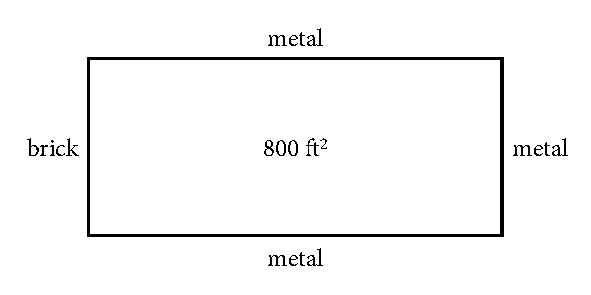
\includegraphics{FinalOptimize}
\newpage
%FTC
 \item The function $f(x)$ has been graphed below.
The curve for $0<x<2$ is an upper half circle.
Define a new function $g(x),$ as
$$
g(x) =\int_0^x f(s)\; ds.
$$

\hfil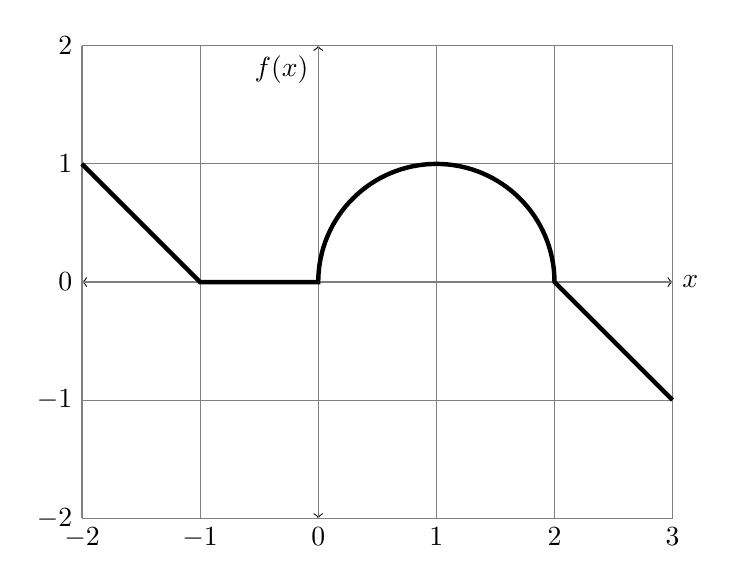
\begin{tikzpicture}[scale=1.5,domain=-3:3]
\draw[<->] (-2,0) -- (3,0) node[right] {$x$};
\draw[<->] (0,-2) -- (0,2) node[below left] {$f(x)$};
\draw[thin,color=gray] (-2,-2) grid (3,2);
\draw[style= ultra thick] (-2,1) --  (-1,0) -- (0,0) arc (180:0:1) -- (3,-1);
\foreach \x in {-2,-1,0,1,2,3}
	\draw (\x,-2) node[below] {$\x$};
\foreach \y in {-2,-1,0,1,2}
	\draw (-2,\y) node[left] {$\y$};
\end{tikzpicture}

Use the graph above to answer the questions below. \\
\textbf{Note:} Pay attention to whether question concerns the function $f$, $f'$, $g$ or $g'.$
\begin{enumerate}
\item  What is the value of $f(0)$?  
\vfill
\item  What is the value of $g(3)$? 
\vfill
\item  What is the value of $g(-2)$? 
\vfill
\item  What is the value of $f'(2)$? 
\vfill
\item  What is the value of $g'(1)$? 
\vfill
\end{enumerate}
\newpage
\item Let $g(x)=\ds\frac{e^{x}}{1+x}.$ Note first and second derivatives are $$g'(x)=\ds\frac{xe^{x}}{(1+x)^{2}} \quad \text{and} \quad g''(x)=\ds\frac{e^{x}(x^{2}+1)}{(1+x)^{3}}.$$ 

Sketch the graph of $g(x).$ Label any asymptotes, $x$- and $y$-intercepts, local minimums and local maximums, and inflection points, if appropriate.\\

\end{enumerate}
\end{document}






